\documentclass[11pt,a4paper]{article}
\usepackage[utf8]{inputenc}
\usepackage[T1]{fontenc}
\usepackage[spanish,es-noshorthands]{babel}
\usepackage{amsmath,amssymb,amsthm}
\usepackage{bm}
\usepackage{geometry}
\geometry{margin=2.5cm}
\usepackage{graphicx}
\graphicspath{{../figuras/}}
\usepackage{float}
\usepackage{xcolor}
\usepackage{hyperref}
\hypersetup{colorlinks=true,linkcolor=blue!50!black,citecolor=blue!50!black,urlcolor=blue!50!black}
\usepackage{enumitem}
\usepackage{booktabs}
\newtheorem{definition}{Definición}
\newtheorem{remark}{Observación}
\newcommand{\R}{\mathbb{R}}
\newcommand{\thetavec}{\bm{\theta}}
\newcommand{\transp}{^{\top}}
\newcommand{\promptIA}[1]{\begin{center}\fcolorbox{gray}{gray!8}{\parbox{0.9\linewidth}{\small\textbf{[FIGURA -- PROMPT IA]}\\[2pt]#1}}\end{center}}
\title{\textbf{Experimentos y resultados}\\[2pt]\large Identificación paramétrica de Wilson--Cowan orientada al control: qué se probó, qué salió y por qué importa}
\author{Proyecto Wilson--Cowan --- Iniciación a la I+D ITBA}
\date{\today}
\begin{document}
\maketitle
\tableofcontents
\bigskip

\section{De qué va este documento}

Este es el documento de \textbf{resultados} del paquete: el recorrido experimental completo del proyecto, de punta a punta. La idea es que se lea como una historia con lógica interna, no como una lista suelta de corridas. Cada experimento aparece con la misma plantilla: \textbf{objetivo} (qué queríamos saber), \textbf{hipótesis} (qué esperábamos y por qué), \textbf{método} (cómo lo medimos), \textbf{resultado} (qué salió) y \textbf{por qué importa} (qué novedad aporta o qué decisión habilita).

El hilo conductor es una sola pregunta y su respuesta incómoda: \emph{¿se pueden recuperar los 10 parámetros de Wilson--Cowan desde datos ruidosos?} La respuesta corta es \emph{casi todos}: hay un parámetro, el peso de autoinhibición $w_{II}$, que se resiste. La gracia del proyecto no es solo detectarlo, sino \textbf{predecirlo antes de entrenar} (con Fisher y SVD), \textbf{mitigarlo} (fijándolo, regularizándolo o rediseñando el estímulo) y, sobre todo, \textbf{mostrar que esa fragilidad no llega al control en lazo cerrado}. Ese último punto (§\ref{sec:control}) es el que da vuelta la lectura pesimista del cuello de botella y es el resultado más importante del paquete.

Recordatorio del modelo (detalle completo en M6, teoría de identificabilidad, y B3, el modelo de Wilson--Cowan). El estado es $\mathbf{x}=[I,E]$, las tasas de disparo (\emph{firing rate}) de las poblaciones inhibitoria y excitatoria; con la sigmoidea $S_a(u)=1/(1+e^{-au})$,
\begin{align}
\dot I &= \tfrac{1}{\tau_i}\big(-I + S_i(w_{IE}E - w_{II}I + Q(t) - \theta_i) - k_i\big),\\
\dot E &= \tfrac{1}{\tau_e}\big(-E + S_e(w_{EE}E - w_{EI}I + P(t) - \theta_e) - k_e\big),
\end{align}
con la salida observada $y(t)=E(t)-I(t)$, los estímulos externos $P(t)\!\to\!E$ y $Q(t)\!\to\!I$, y los offsets $k_e,k_i$ derivados (no aprendidos) para que el reposo sea equilibrio. Los 10 parámetros a identificar son $\thetavec=(w_{EE},w_{EI},w_{IE},w_{II},\tau_e,\tau_i,a_e,a_i,\theta_e,\theta_i)$. El régimen objetivo es \emph{theta-gamma}, y los estímulos se piensan realizables con optogenética (on/off, $\ge 0$).

\begin{remark}
Todas las figuras de este documento son resultados reales del proyecto (llevan la nota \emph{(figura del proyecto)} en el epígrafe). El detalle de métodos de identificación está en M5; el diagnóstico de identificabilidad (Fisher, SVD, Cramér--Rao, OED) en M6; el análisis de control en B5.
\end{remark}

\section{Simulador y datasets sintéticos}
\label{sec:sim}

\paragraph{Objetivo.} Construir el ``cerebro de mentira'' \--- un simulador de Wilson--Cowan del que conocemos la verdad de terreno (\emph{ground truth}) \--- y generar los datasets con distintos estímulos y niveles de ruido sobre los que se hará toda la identificación. Sin un simulador confiable no hay experimento posible: es el banco de pruebas de todo el resto.

\paragraph{Método.} Se integra WC con RK45 adaptativo (tolerancia estricta, \texttt{rtol}$\approx 10^{-11}$) para tener trayectorias de referencia limpias. Alrededor se arma una \textbf{librería de estímulos}: pulsos, \emph{chirp} (barrido de frecuencia), APRBS/PRBS (señales binarias pseudoaleatorias), theta-gamma, Poisson y onda cuadrada, aplicando $P$ a la población $E$ y $Q$ a la $I$. Sobre las trayectorias limpias se agrega ruido de observación gaussiano con desvío $\sigma$ para simular medición realista.

Los datasets concretos: un conjunto de control (\texttt{multi\_dataset.npz}, 19 trayectorias $\times$ 2000 pasos) y los de identificación (12 escenarios, 8 de entrenamiento y 4 de test, 4000 pasos cada uno con $dt\approx0.05$ sobre $T=(0,200)$).

\begin{figure}[H]\centering
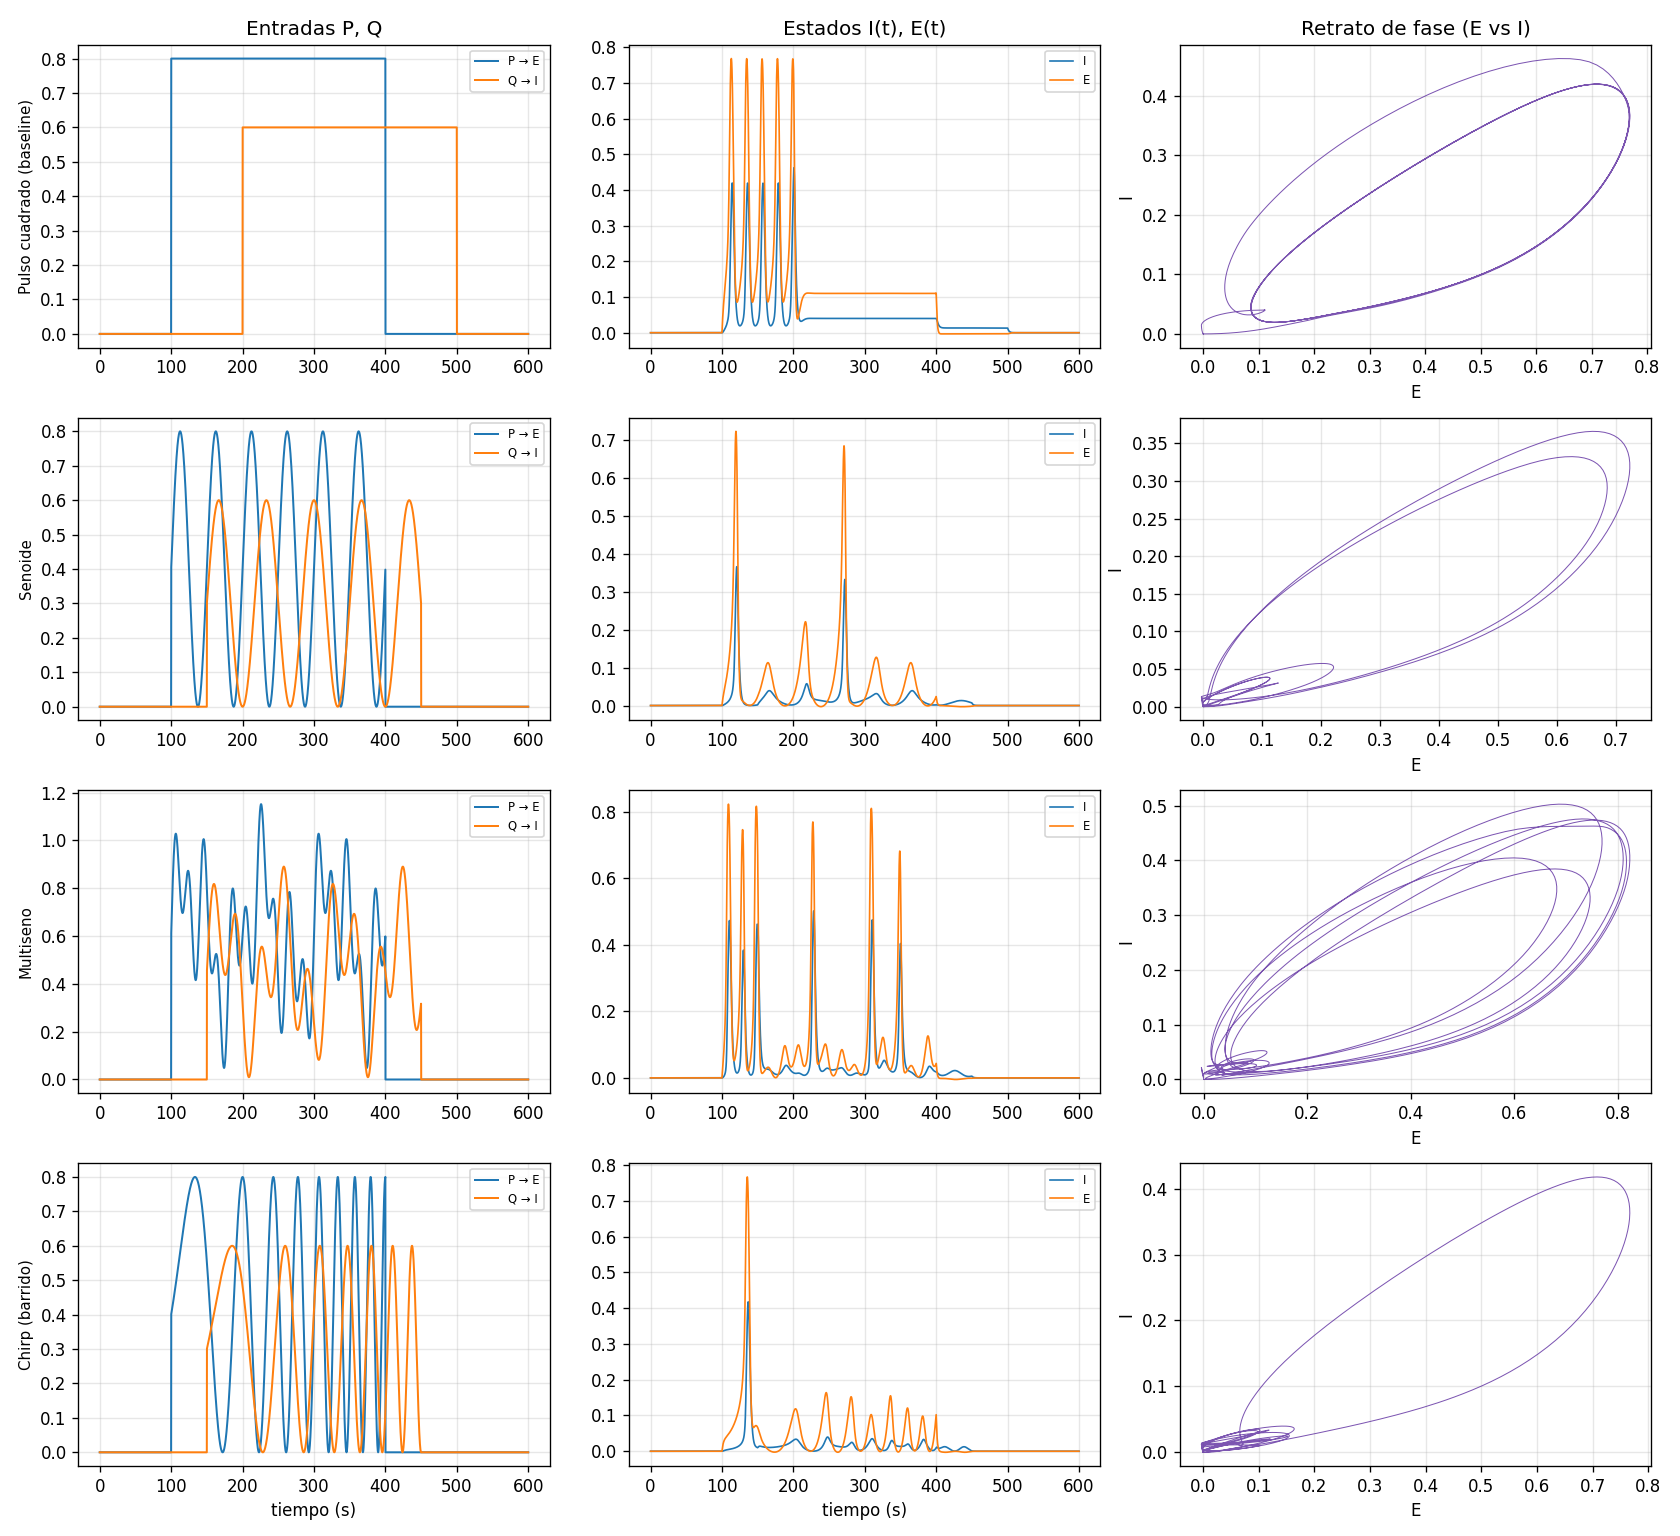
\includegraphics[width=0.75\linewidth]{demo_estimulos.png}
\caption{Cobertura del espacio de estados por familia de estímulo: cada tipo de entrada empuja al sistema por regiones distintas del plano $(I,E)$. \emph{(figura del proyecto)}}
\label{fig:demo}
\end{figure}

\paragraph{Por qué importa.} La diversidad de estímulos no es un capricho: es el principio de \textbf{excitación persistente} de la identificación de sistemas (Ljung 1999 \cite{ljung}). Distintas entradas vuelven identificables distintos parámetros, porque cada una hace ``vibrar'' al sistema en direcciones diferentes del espacio de parámetros. Esta intuición, que acá aparece como una figura de cobertura, es exactamente la que después se formaliza con la matriz de información de Fisher y se explota en el diseño de experimentos (§\ref{sec:oed}). El simulador con \emph{ground truth} conocido es lo que nos permite medir error real de identificación \--- un lujo que con datos biológicos reales no tendríamos.

\section{Identificación en limpio: 4 pesos y luego los 10 parámetros}
\label{sec:limpio}

\paragraph{Objetivo.} Recuperar los parámetros de WC desde trayectorias \textbf{sin ruido}. Es la línea de base que después no hay que empeorar: si el método no funciona en el caso ideal, no tiene sentido pelear con el ruido.

\paragraph{Hipótesis.} Con excitación rica (varias familias de estímulo) y varias trayectorias, los pesos son identificables con error bajo. La pregunta abierta era hasta dónde escala: ¿los 4 pesos sinápticos solamente, o los 10 parámetros completos?

\paragraph{Método.} Dos arquitecturas de SciML, comparadas en M5: una \textbf{PINN} (aprende la solución $t\mapsto x$, con \emph{Fourier features} para no perder alta frecuencia) y una \textbf{Neural ODE} (aprende la dinámica $(x,P,Q)\mapsto\dot x$ e integra con RK4 diferenciable, usando \emph{multiple shooting} en ventanas de 100 pasos). Ambas evitan estimar derivadas de los datos \--- la debilidad del baseline clásico tipo SINDy \--- y por eso son más robustas al ruido. La NODE se entrena con Adam (2000--3000 épocas) más un pulido final con L-BFGS.

\paragraph{Resultado.} En limpio, los \textbf{4 pesos} se recuperan casi perfecto: la Neural ODE llega a $0.42\%$ de error y la PINN a $\le 1.7\%$. El salto importante es la extensión a los \textbf{10 parámetros} con la Neural ODE, arrancando desde una inicialización ignorante (sin conocer los valores verdaderos): \textbf{error máximo $1.14\%$} sobre los diez. La Figura~\ref{fig:fit_joint} muestra el ajuste conjunto y la Figura~\ref{fig:conv} la convergencia del entrenamiento. La Figura~\ref{fig:chirp} es la prueba de fuego: se simula WC con los parámetros identificados frente al WC verdadero sobre una trayectoria \emph{chirp} \textbf{no vista en entrenamiento}; el solapamiento es casi total.

\begin{figure}[H]\centering
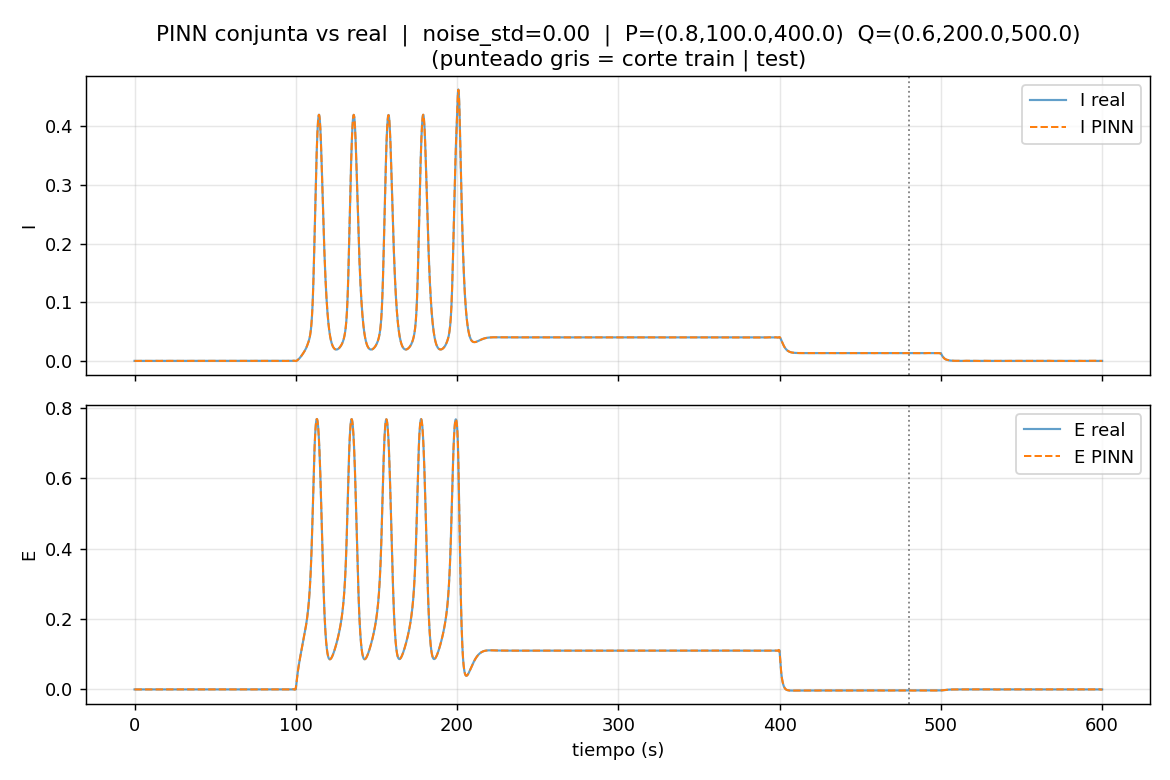
\includegraphics[width=0.75\linewidth]{fit_joint_noise_0_00.png}
\caption{Identificación conjunta de los 10 parámetros en limpio ($\sigma=0$): ajuste sobre las trayectorias. \emph{(figura del proyecto)}}
\label{fig:fit_joint}
\end{figure}

\begin{figure}[H]\centering
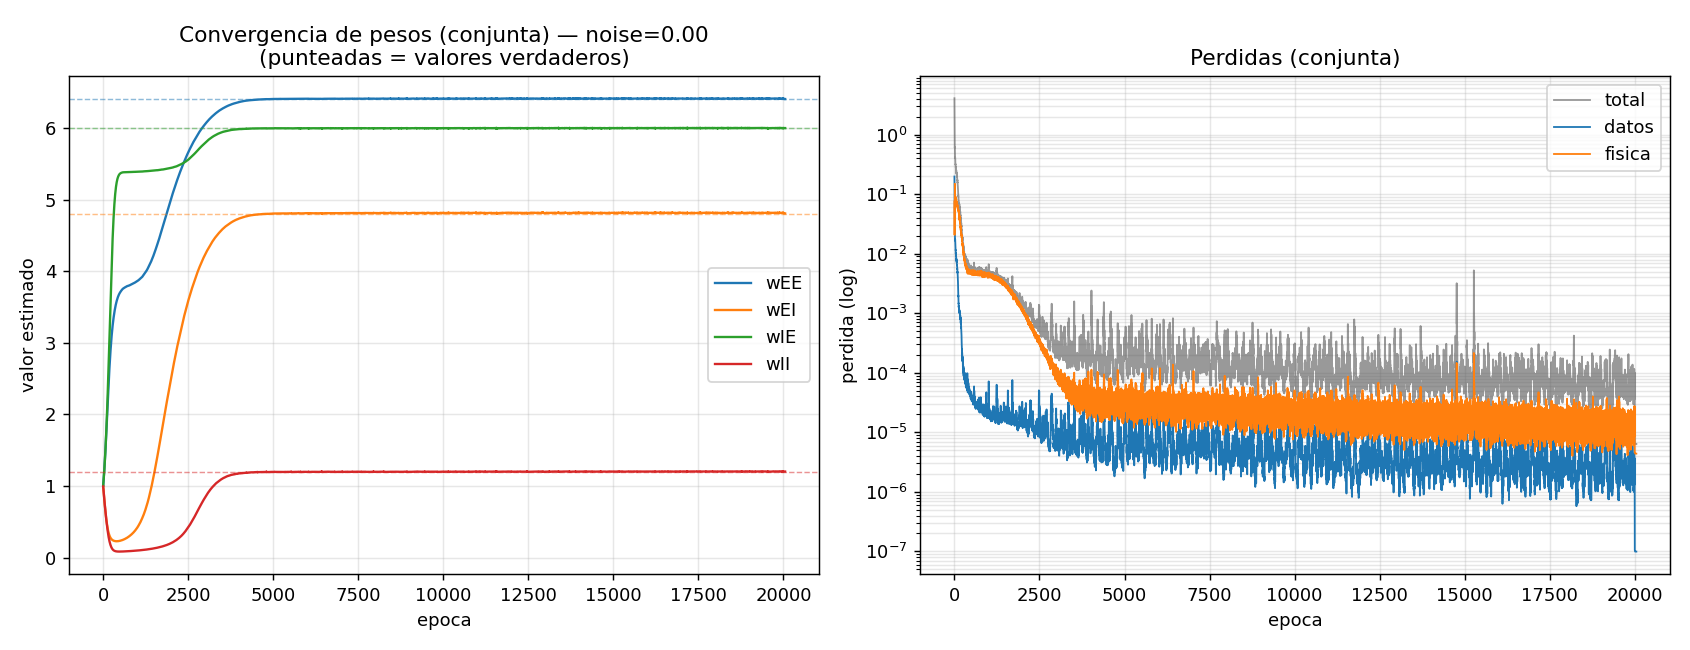
\includegraphics[width=0.75\linewidth]{convergencia_joint_noise_0_00.png}
\caption{Convergencia del entrenamiento de la identificación conjunta (10 parámetros, $\sigma=0$); la pérdida cae hasta estabilizarse cerca de la época 1250. \emph{(figura del proyecto)}}
\label{fig:conv}
\end{figure}

\begin{figure}[H]\centering
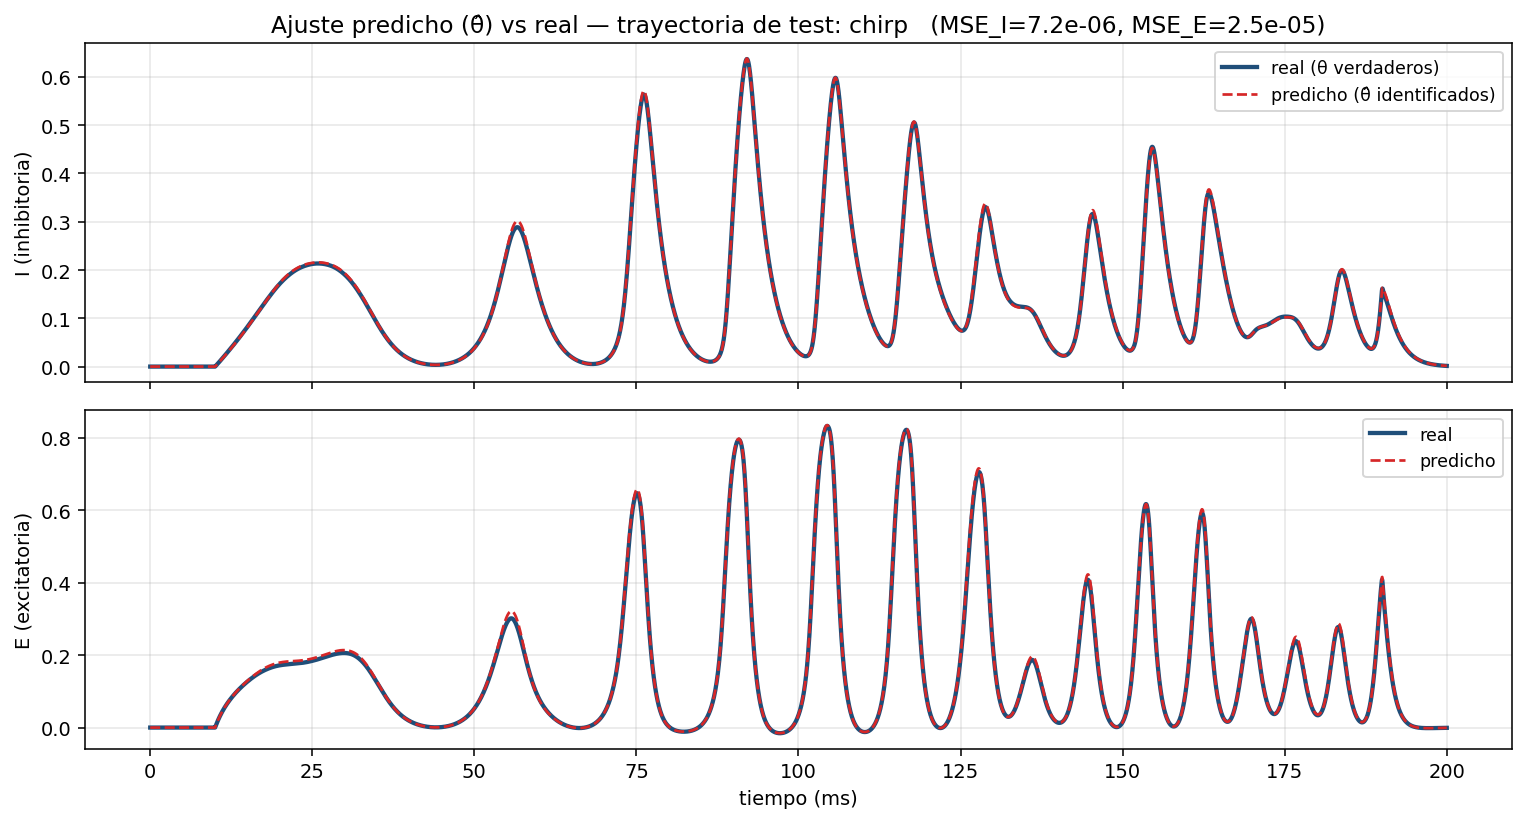
\includegraphics[width=0.75\linewidth]{fit_chirp_test.png}
\caption{Reconstrucción sobre test tipo \emph{chirp} (estímulo no visto): WC con los parámetros identificados vs.\ WC verdadero. El solapamiento casi total ilustra la calidad de la identificación limpia. \emph{(figura del proyecto)}}
\label{fig:chirp}
\end{figure}

\paragraph{Por qué importa.} La \textbf{novedad} está en identificar los \textbf{10 parámetros} de Wilson--Cowan con una Neural ODE, no solo los 4 pesos sinápticos \--- no encontramos esto hecho en la literatura (más en M6 y en la discusión de trabajo relacionado). Y, más práctico: este experimento fija la referencia contra la cual medir toda la degradación posterior. Si en limpio el peor parámetro tiene $1.14\%$ de error y bajo ruido salta a $41\%$, ese contraste es toda la historia del cuello de botella. La identificación limpia es, además, la condición necesaria para el control: solo tiene sentido preguntar si los $\hat\theta$ sirven para controlar (§\ref{sec:control}) una vez que sabemos que se pueden recuperar bien en el caso ideal.

\section{Robustez al ruido y diagnóstico Fisher\,+\,SVD}
\label{sec:ruido}

\paragraph{Objetivo.} Averiguar qué se puede recuperar \textbf{bajo ruido de observación}. Los datos reales no son limpios, y la pregunta clave es si la degradación golpea a todos los parámetros por igual o si hay unos más frágiles que otros.

\paragraph{Hipótesis (predicha \emph{antes} de entrenar).} Este es el punto metodológicamente más lindo. Antes de tocar ninguna red, la teoría de identificabilidad hace una predicción concreta. La \textbf{matriz de sensibilidad} $J=\partial y/\partial\thetavec$ mide cuánto cambia la trayectoria al mover cada parámetro; su producto $J\transp J$ (proporcional a la \textbf{matriz de información de Fisher}, FIM) tiene autovalores que son los valores singulares de $J$ al cuadrado. Un autovalor chico es una \textbf{dirección plana}: una combinación de parámetros que casi no deja huella en los datos y, por lo tanto, no se puede identificar. La cota de Cramér--Rao,
\begin{equation}
\mathrm{std}(\hat\theta_j)\ \ge\ \sigma_\varepsilon\sqrt{[(J\transp J)^{-1}]_{jj}},
\end{equation}
convierte eso en el mejor error posible por parámetro. La FIM predijo una dirección plana dominada por $\bm{w_{II}}$ (acoplada con $a_e$--$\tau_e$--$w_{EE}$ y $a_i$--$\tau_i$--$\theta_i$). Hipótesis: \textbf{$w_{II}$ será el peor identificado}.

\paragraph{Método.} Barrido de ruido $\sigma\in\{0,\,0.01,\,0.05,\,0.10\}$ sobre 12 trayectorias (8 train / 4 test, 4000 pasos), con suavizado adaptativo (ventana $k=7\to11$) y estímulo fuerte ($Q$ grande) para maximizar la información disponible. Se identifican los 10 parámetros con la Neural ODE en cada nivel de ruido.

\paragraph{Resultado.} La predicción \textbf{se confirma casi exacta}. La degradación es fuertemente \textbf{no uniforme} y sigue el ranking que marcó la FIM:
\begin{itemize}[leftmargin=1.4em,itemsep=1pt]
\item \textbf{$w_{II}$ es el peor a todos los niveles}: de $0.8\%$ en limpio salta a $\mathbf{41\%}$ a $\sigma=0.10$ (la dirección singular más débil).
\item Le siguen los del acople que marcó la SVD: $\tau_i$ ($15.9\%$), $a_i$ ($11.5\%$), $a_e$ ($9.1\%$).
\item Los \textbf{mejor identificados} son $w_{IE}$ ($1.2\%$), $w_{EE}$ ($3.3\%$) y $\theta_e$ ($4.0\%$) \--- también como anticipó la sensibilidad.
\end{itemize}
Hay además un hallazgo secundario importante: \textbf{identificar los 10 es mucho menos robusto que identificar solo los 4 pesos}. A $\sigma=0.10$ el peor de los 10 llega a $41\%$ ($w_{II}$) contra $8.9\%$ si solo se estiman los 4 pesos. Liberar $a_i$, $\tau_i$ y $\theta_i$ \--- que compiten con $w_{II}$ en la ecuación de $I$ \--- le ``roba'' identificabilidad a $w_{II}$. La Figura~\ref{fig:noise} muestra el error por parámetro contra el nivel de ruido.

\begin{figure}[H]\centering
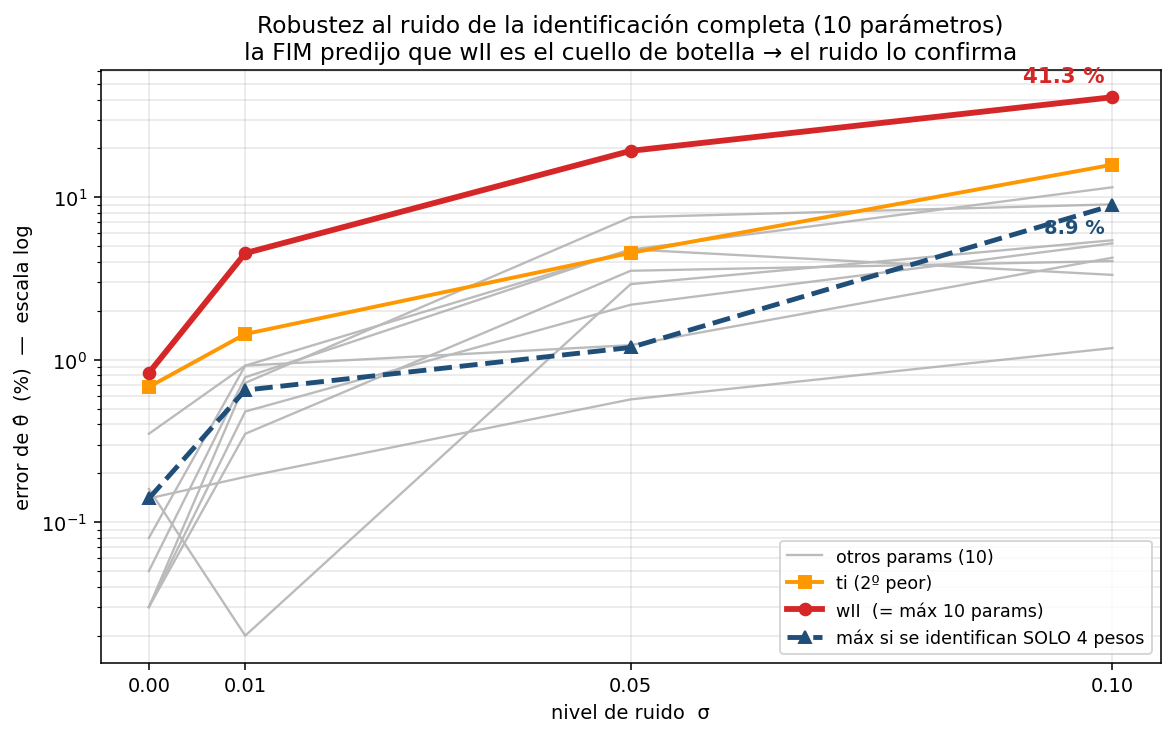
\includegraphics[width=0.8\linewidth]{noise_param_error.png}
\caption{Error de identificación por parámetro vs.\ nivel de ruido $\sigma$. $w_{II}$ se despega del resto y explota a $\sigma=0.10$, siguiendo el ranking predicho por la FIM. \emph{(figura del proyecto)}}
\label{fig:noise}
\end{figure}

\paragraph{Por qué importa.} La novedad es el bucle \textbf{predecir $\to$ confirmar}: la FIM anticipa que $w_{II}$ es el cuello de botella \emph{sin entrenar nada}, y el ruido lo verifica. Esto no es una anécdota metodológica: significa que, frente a cualquier modelo nuevo o dataset nuevo, podemos saber \textbf{de antemano} qué parámetros van a costar, sin gastar horas de cómputo probando. Es la misma lógica que después se repite con el costo computacional (§\ref{sec:costo}): un espectro de un Jacobiano predice el comportamiento. El detalle teórico está en M6.

\section{Remedios guiados por la FIM}
\label{sec:remedios}

\paragraph{Objetivo.} Mitigar la mala identificabilidad de $w_{II}$. Si ya sabemos cuál es el problema y por qué, la pregunta es qué hacer al respecto.

\paragraph{Hipótesis.} Fijar el parámetro mal condicionado debería \textbf{liberar} a los demás (sacarle la competencia), y los estímulos de banda ancha deberían condicionar mejor la FIM.

\paragraph{Método y teoría.} Se aplican tres herramientas estándar de identificabilidad, todas prestadas y citadas (M6):
\begin{itemize}[leftmargin=1.4em,itemsep=2pt]
\item \textbf{Subset selection} por QR con pivoteo (Chu \& Hahn 2007 \cite{chuhahn}): elige qué parámetro conviene fijar.
\item \textbf{Regularización} de Tikhonov / MAP: penaliza el alejamiento de $w_{II}$ de un valor de referencia con fuerza $\lambda$; en el límite $\lambda\to\infty$ equivale a fijarlo. La conexión con \emph{profile likelihood} es Raue 2009 \cite{raue}.
\item \textbf{OED} (diseño óptimo de experimentos): criterios A/D/E-óptimos sobre la FIM (Ljung 1999 \cite{ljung}).
\end{itemize}
Se corre sobre los 12 escenarios a $\sigma=0.10$; el análisis OED por familia se hace incluso \textbf{sin entrenar}, calculando la FIM por diferenciación automática (\texttt{jacfwd}) sobre 7 familias de estímulo.

\paragraph{Resultado.}
\begin{description}[leftmargin=0pt,itemsep=4pt]
\item[(A) Fijar o regularizar $w_{II}$.] \emph{Fijar} $w_{II}$ en su valor verdadero (que conocemos en el setup sintético) y re-identificar los otros 9 baja el error del resto de $15.9\%$ a $\mathbf{9.7\%}$ a $\sigma=0.10$; los que más mejoran son justamente $\tau_i$, $a_i$ y $\theta_i$ (los del acople). \emph{Regularizar} da el \textbf{continuo} entre libre y fijo: el error baja monótono con $\lambda$ y \textbf{satura en el mismo $9.7\%$} cuando $\lambda\to\infty$, con un óptimo práctico en $\lambda\approx1.0$. Figuras~\ref{fig:fixwii} y~\ref{fig:reglambda}.
\item[(B) Qué fijar (QR-pivoteo).] Fijar $w_{II}$ o $a_i$ es casi óptimo; fijar $a_e$ es inútil; y fijar $w_{II}$ \textbf{y} $a_i$ \emph{juntos} es contraproducente ($99.7\%$ de error). Lección: hay que fijar un \textbf{representante mínimo} del acople, no varios miembros de la misma dirección plana. Figura~\ref{fig:heatmap}.
\item[(C) OED por familia.] Los estímulos de banda ancha (\emph{chirp}, Poisson) condicionan la FIM mucho mejor que los tipo caja o cuadrada, por \textbf{decorrelación} de $E$ e $I$. Y la métrica correcta para comparar estímulos es Cramér--Rao, no la norma de la columna de sensibilidad. Figura~\ref{fig:oedfam}.
\end{description}

\begin{figure}[H]\centering
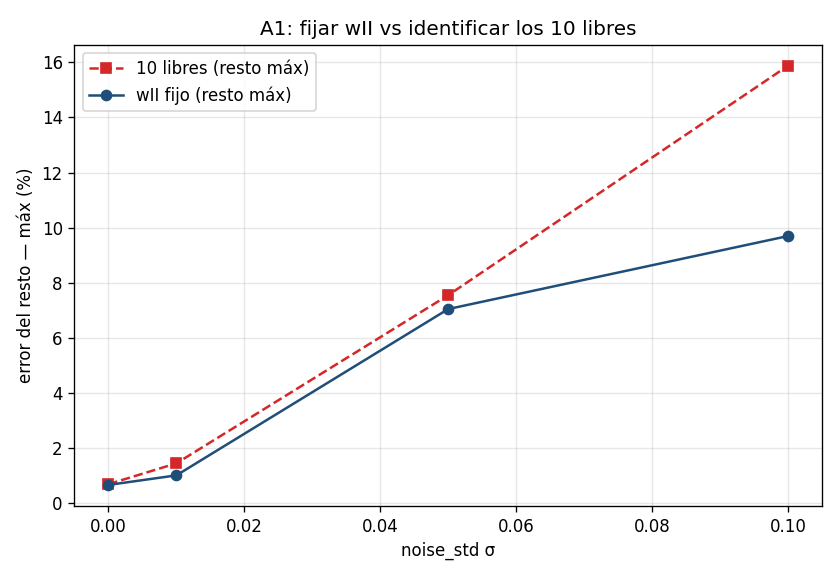
\includegraphics[width=0.7\linewidth]{expA1_fix_wII.png}
\caption{Efecto de fijar $w_{II}$ en su valor verdadero: el error del resto de los parámetros baja de $15.9\%$ a $9.7\%$ ($\sigma=0.10$). \emph{(figura del proyecto)}}
\label{fig:fixwii}
\end{figure}

\begin{figure}[H]\centering
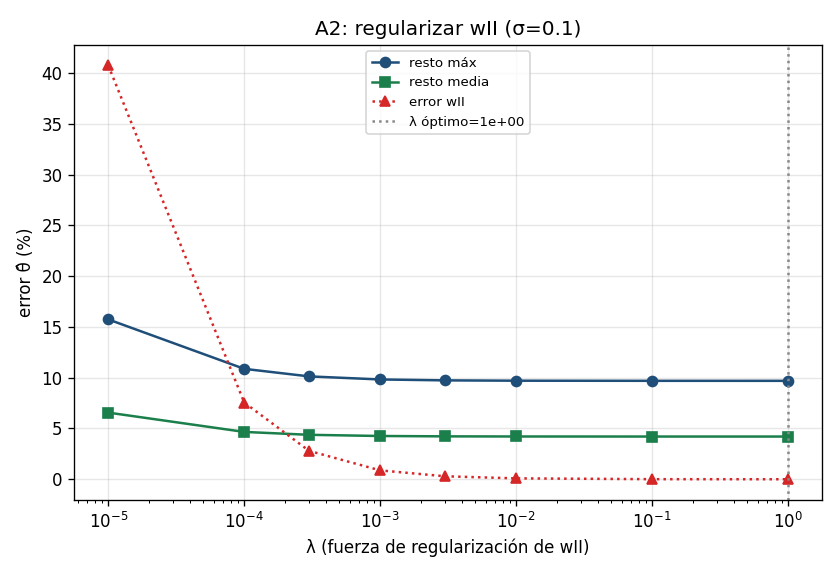
\includegraphics[width=0.7\linewidth]{expA2_reg_lambda.png}
\caption{Barrido de la fuerza de regularización $\lambda$ sobre $w_{II}$: el error del resto baja monótono y satura en el mismo $9.7\%$ que ``fijar'' ($\lambda\to\infty$). \emph{(figura del proyecto)}}
\label{fig:reglambda}
\end{figure}

\begin{figure}[H]\centering
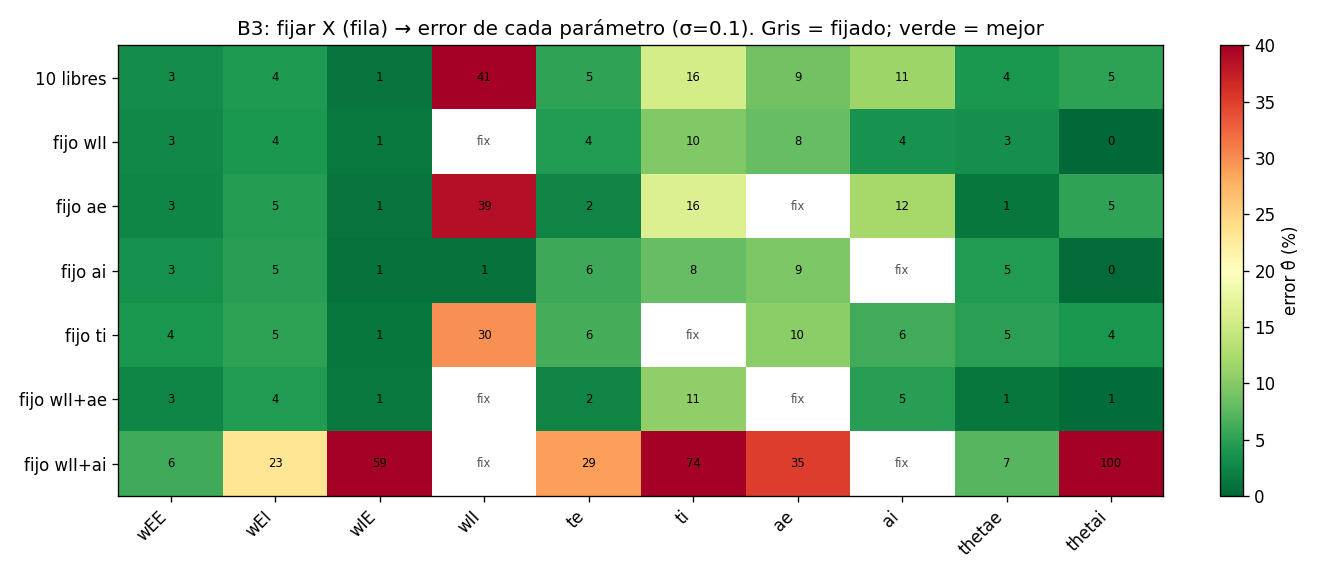
\includegraphics[width=0.7\linewidth]{expB_heatmap_fijar.png}
\caption{Qué conviene fijar (QR-pivoteo): fijar $w_{II}$ o $a_i$ es casi óptimo; fijar dos miembros del mismo acople es contraproducente. \emph{(figura del proyecto)}}
\label{fig:heatmap}
\end{figure}

\begin{figure}[H]\centering
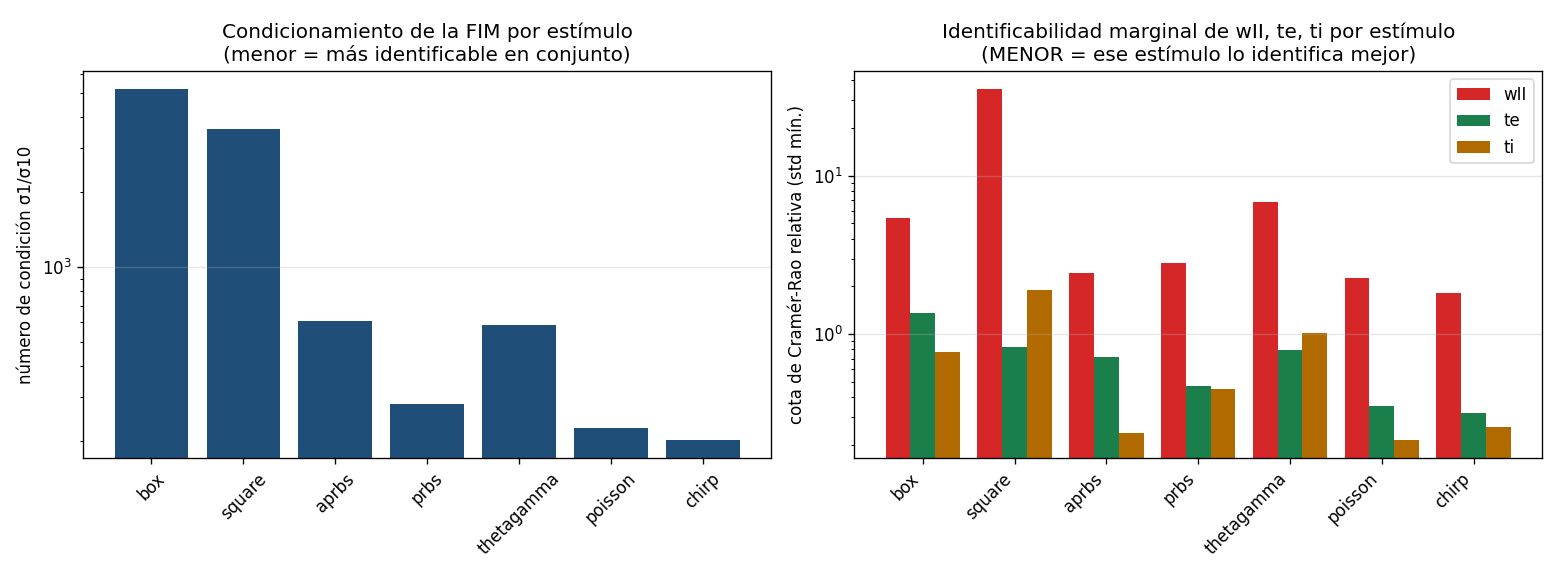
\includegraphics[width=0.7\linewidth]{oed_cond_por_estimulo.png}
\caption{Número de condición de la FIM por familia de estímulo: los estímulos de banda ancha (\emph{chirp}, Poisson) condicionan mucho mejor que los tipo caja. \emph{(figura del proyecto)}}
\label{fig:oedfam}
\end{figure}

\paragraph{Por qué importa.} Los métodos son prestados, pero la \textbf{aplicación conjunta a Wilson--Cowan identificado con Neural ODE} \--- con el hallazgo concreto ($w_{II}$) y una receta accionable (fijar un representante mínimo, regularizar con $\lambda\approx1$, elegir estímulos de banda ancha) \--- es la contribución. Además, el resultado (B) es contraintuitivo y útil: más restricciones no es mejor; fijar de más rompe el ajuste. Eso solo se ve porque la SVD nos dice cuáles parámetros viven en la misma dirección plana.

\section{OED ponderado al cuello de botella}
\label{sec:oed}

\paragraph{Objetivo.} Diseñar el dataset que mejor identifica específicamente a $w_{II}$. El experimento anterior (C) mostró que la familia de estímulo importa, pero dejó abierta una pregunta: el OED debería \textbf{ponderar hacia el parámetro peor identificado}, no solo repartir cobertura de forma uniforme.

\paragraph{Conceptos clave.} Dos ingredientes, y hacen falta los dos:
\begin{itemize}[leftmargin=1.4em,itemsep=2pt]
\item \textbf{Decorrelación}: usar \emph{chirp} con $P$ y $Q$ en \textbf{bandas de frecuencia distintas}, para que $E$ e $I$ no se muevan juntos. Si $E\approx I$, los términos de acople $w_{IE}E$ y $w_{II}I$ quedan casi colineales y el ajuste no los distingue. Decorrelar \textbf{separa} $w_{II}$ de $w_{IE}$.
\item \textbf{Q-alta}: amplitud grande en el estímulo $Q$ (entrada a $I$). Como $w_{II}$ multiplica a $I$, excitar fuerte a $I$ hace que $w_{II}$ deje más huella. Q-alta \textbf{hace visible} a $w_{II}$ (mejora el SNR).
\end{itemize}
En una frase: \emph{decorrelación separa, Q-alta hace visible.}

\paragraph{Hipótesis.} Existe un balance \textbf{intermedio óptimo}: ni solo decorrelación (con $w_{II}$ poco visible) ni solo Q-alta (con $w_{II}$ colineal con $w_{IE}$) alcanzan por sí solas.

\paragraph{Método.} Barrido de la proporción $\rho$ = fracción de trayectorias Q-alta vs.\ de decorrelación (8 trayectorias \emph{chirp} por dataset, componentes suaves para conservar el $dt$ grande, $\sigma=0.10$). Cinco proporciones $\times$ tres semillas $=$ 15 corridas.

\paragraph{Resultado.} \textbf{V-shape con óptimo en $\rho=0.5$} (4 trayectorias Q-alta + 4 de decorrelación): el error de $w_{II}$ baja a $\mathbf{18.7\%}$, contra $93\%$ con solo decorrelación y $98.7\%$ con solo Q-alta. Confirma la hipótesis: hacen falta las dos cosas a la vez. La Figura~\ref{fig:oedw} muestra la V.

\begin{figure}[H]\centering
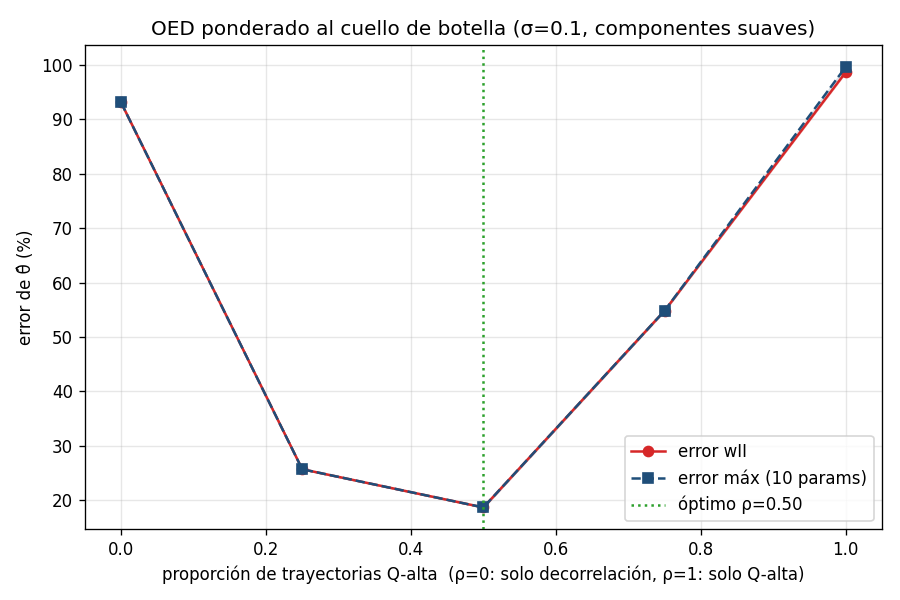
\includegraphics[width=0.7\linewidth]{oed_weighted.png}
\caption{OED ponderado al cuello de botella: error de $w_{II}$ vs.\ proporción $\rho$ de trayectorias Q-alta. V-shape con óptimo en $\rho=0.5$. \emph{(figura del proyecto)}}
\label{fig:oedw}
\end{figure}

\paragraph{Limitaciones y cómo mejorarlo.} Honestidad ante todo: (i) el \emph{chirp} no es realizable con optogenética (on/off), así que la versión implementable debería repetirse con estímulos conmutados (PRBS/APRBS para decorrelación + trenes de pulsos de gran amplitud para Q-alta), y esos requieren $dt$ fino (§\ref{sec:familia}); (ii) las tres semillas salieron redundantes, así que no hay barras de error reales \--- habría que variar la realización del ruido entre corridas; (iii) convendría una grilla más fina de $\rho$ cerca de $0.5$. Lo esperado en todos los casos es que la V-shape persista, aunque desplazada.

\paragraph{Por qué importa.} La novedad es aplicar diseño óptimo de experimentos y excitación persistente (Ljung 1999 \cite{ljung}; Plate 2024 \cite{plate}) a WC con Neural ODE \textbf{ponderando explícitamente hacia el parámetro cuello de botella}, y verificarlo empíricamente (la V). Es el paso de ``sabemos que $w_{II}$ es difícil'' a ``sabemos cómo diseñar el experimento para hacerlo menos difícil''.

\section{Identificación por familia y el límite del \emph{dt} grande}
\label{sec:familia}

\paragraph{Objetivo.} Comprobar si la Neural ODE, entrenada \textbf{por familia de estímulo}, confirma el ranking de identificabilidad que predijo la cota de Cramér--Rao. Cerrar el triángulo: PINN-por-familia + NODE-sobre-mezcla + OED.

\paragraph{Método.} Cinco familias $\times$ cuatro trayectorias, $\sigma=0.05$, en dos corridas: una con $dt$ grande ($N_{\text{eval}}=1000$, ventana 25) y otra con $dt$ fino ($N_{\text{eval}}=4000$, ventana 100).

\paragraph{Resultado: no concluyente.} A $dt$ grande solo el \emph{chirp} (suave) identificó bien; a $dt$ fino se recuperaron aprbs y theta-gamma, pero el \emph{chirp} empeoró. La causa es una mezcla de varianza de optimización alta y estímulos no comparables a los que usó la CRB. La Figura~\ref{fig:family} muestra la comparación.

\begin{figure}[H]\centering
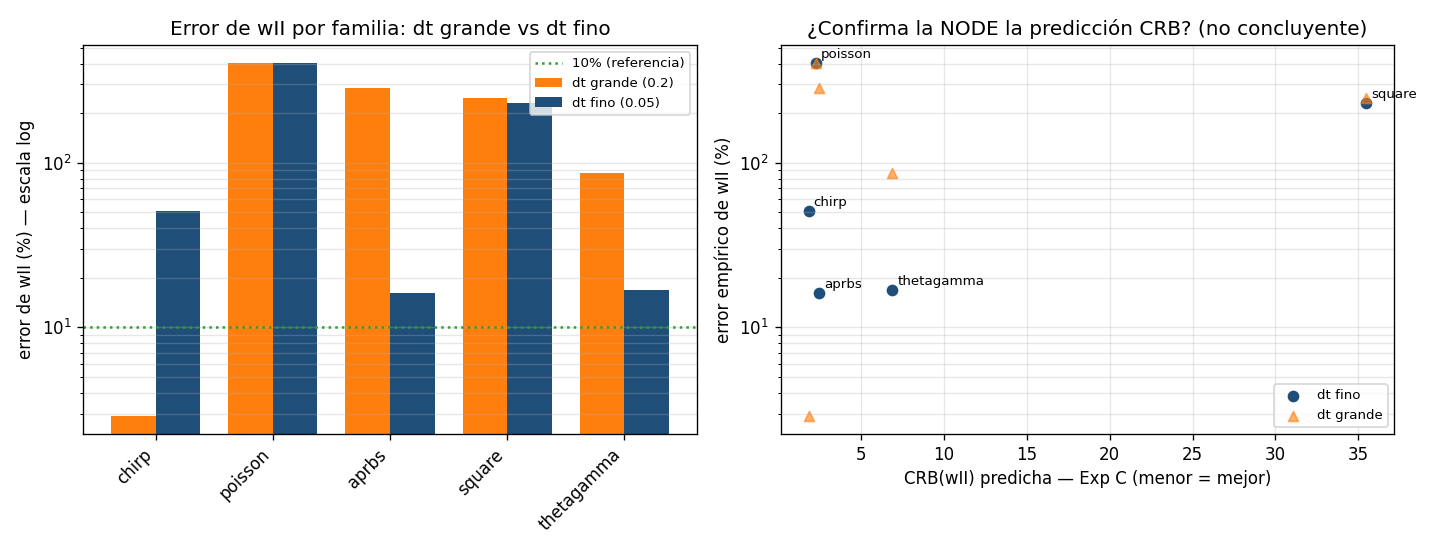
\includegraphics[width=0.8\linewidth]{family_compare_dt.png}
\caption{Identificación NODE por familia con $dt$ grande vs.\ $dt$ fino: resultado no concluyente, pero deja firme que el $dt$ grande solo es seguro con estímulos suaves. \emph{(figura del proyecto)}}
\label{fig:family}
\end{figure}

\paragraph{Por qué importa.} Aunque no cierra el triángulo, deja un resultado metodológico \textbf{firme}: el \textbf{$dt$ grande solo es seguro para estímulos suaves} (\emph{chirp}); los conmutados (on/off) necesitan $dt$ fino porque sus transiciones bruscas rompen la integración con paso grande. Esto es rigor: en vez de reportar un número dudoso, identificamos el confusor. Y tiene consecuencia directa en el experimento anterior (§\ref{sec:oed}) y en el de costo (§\ref{sec:costo}): la palanca del $dt$ grande, que abarata todo, tiene un límite conocido.

\section{Costo computacional}
\label{sec:costo}

\paragraph{Objetivo.} Cuantificar cuánto cuesta identificar y cómo abaratarlo sin perder calidad. Y una pregunta más ambiciosa: ¿hay un \textbf{estimador a priori} del costo, como Fisher+SVD lo es de la identificabilidad?

\paragraph{Hipótesis.} Sí: la \textbf{rigidez} del sistema \--- los autovalores del Jacobiano de estado $\partial f/\partial x$ \--- predice el paso de integración estable, y por lo tanto el costo, sin necesidad de correr nada.

\paragraph{Método.} Este experimento \textbf{no entrena}: integra la dinámica conocida. Se toma como referencia scipy RK45 (tolerancia $10^{-11}$, 3001 puntos) y se hace un barrido de $dt\in\{0.05\dots2.0\}$ cruzado con solvers Euler / RK2 / RK4; la rigidez se mide con los autovalores de $\partial f/\partial x$ en 200 puntos de la trayectoria.

\paragraph{La matemática, concisa.} El paso explícito estable cumple $\Delta t\cdot|\lambda_{\max}|\lesssim 2.78$ (región de estabilidad de RK4 sobre el eje real). En WC $|\lambda_{\max}|\approx0.70$, así que $\Delta t$ estable $\approx 2.78/0.70\approx4.0$. Y como el ratio $|\lambda_{\max}|/|\lambda_{\min}|\approx1$ (nada rígido), no hay transitorios rápidos a los que ``adaptarse'', de modo que el paso adaptativo casi no gana frente a un paso fijo grande.

\paragraph{Resultado.} \textbf{WC no es rígido} ($|\lambda_{\max}|\approx0.70$). Por eso RK4 con $\Delta t$ grande (NFE $\approx600$) da la misma precisión práctica que el adaptativo (nfev $\approx3050$) $\to$ \textbf{unas 5 veces más barato}. Y, lo importante, la rigidez lo \textbf{predice sin correr nada}. La Figura~\ref{fig:cost} muestra el barrido. En números concretos de entrenamiento, bajar $\Delta t$ de $0.05$ a $0.2$ (con estímulos suaves) redujo el tiempo por época de $\sim510$ ms a $\sim140$ ms ($\sim3.7\times$), y bajar de 6000 a 2000 épocas (converge $\sim$1250) sumó otro $3\times$.

\begin{figure}[H]\centering
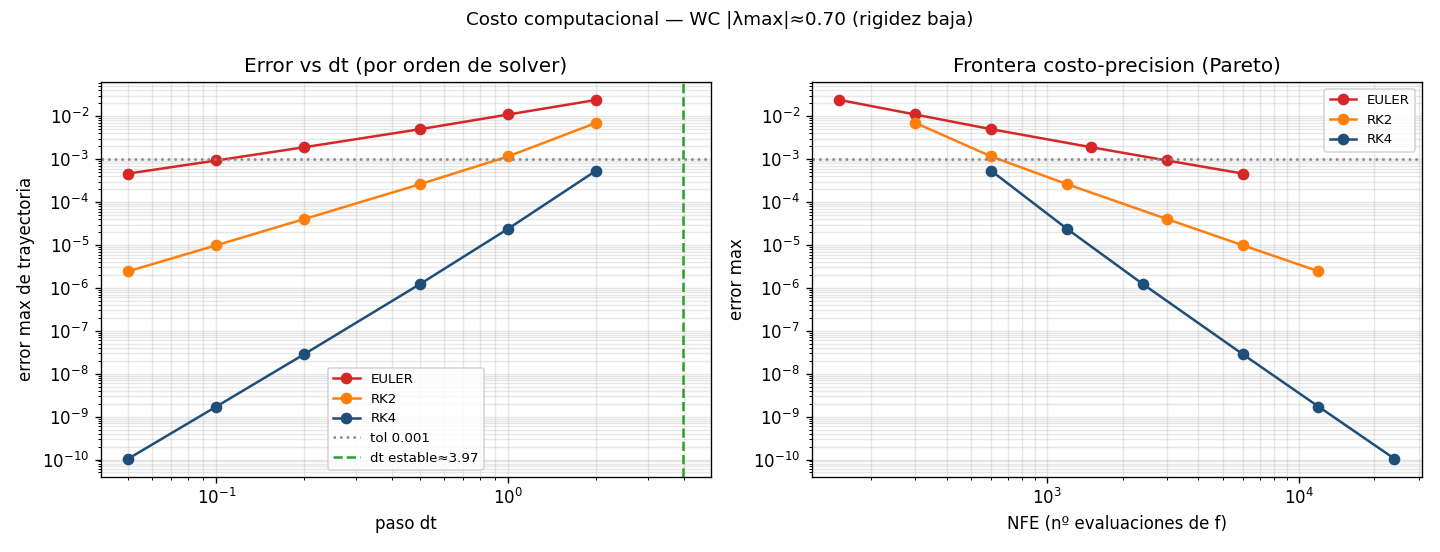
\includegraphics[width=0.8\linewidth]{cost_dt_sweep.png}
\caption{Costo computacional vs.\ paso de integración $dt$ y solver: RK4 con $dt$ grande alcanza la precisión del adaptativo a una fracción del costo. \emph{(figura del proyecto)}}
\label{fig:cost}
\end{figure}

\paragraph{Por qué importa.} La \textbf{novedad conceptual} es la simetría: la rigidez es el gemelo computacional del número de condición de la FIM. Una predice \textbf{costo}, la otra \textbf{identificabilidad}; ambas son espectros de un Jacobiano ($\partial f/\partial x$ contra $\partial y/\partial\thetavec$). Los dos análisis caros del proyecto \--- ¿qué puedo recuperar? y ¿cuánto me va a costar? \--- se responden mirando autovalores de un Jacobiano \emph{antes} de gastar cómputo. Ese es el hilo que une §\ref{sec:ruido} con esta sección.

\section{Validación orientada al control}
\label{sec:control}

\paragraph{Objetivo.} La pregunta que justifica todo el proyecto: ¿sirven los parámetros identificados $\hat\theta$ para \textbf{controlar} el sistema? Y, específicamente, ¿la fragilidad de la identificación (ese $w_{II}$ que a $\sigma=0.10$ tiene $41\%$ de error) rompe el control?

\paragraph{Motivación.} Es el objetivo final: la cadena completa \emph{identificar $\to$ controlar}. Todo el análisis anterior sería una curiosidad académica si la fragilidad de $w_{II}$ hiciera inservible al modelo identificado como planta de un controlador.

\paragraph{Hipótesis.} La \textbf{acción integral} del controlador IMC absorbe el error de modelo, de modo que el control resulta \textbf{más robusto que la identificación}. La intuición: el IMC usa los pesos ($\hat\theta$) para la cancelación por linealización, pero la realimentación integral corrige el residuo sin depender de $\hat\theta$.

\paragraph{Método.} Simulación en lazo cerrado con RK4 ($dt=0.005$ ms, $t_f=50$ ms, $\sim$10\,000 pasos), sobre una matriz $2\times2$ de \{simulador, Neural ODE\} $\times$ \{$\hat\theta$, parámetros reales\}, barriendo el ruido $\sigma\in\{0,0.01,0.05,0.10\}$. Se compara el RMSE de seguimiento del ritmo objetivo. El controlador se describe en B5.

\paragraph{Resultado.} El RMSE de seguimiento es \textbf{casi idéntico} con $\hat\theta$ que con los parámetros reales, y se mantiene cerca del ideal \textbf{incluso con $\hat\theta$ muy degradado bajo ruido} (por ejemplo, con $w_{II}$ lejos de su valor verdadero). \textbf{La fragilidad de la identificación no se propaga al control.} La Figura~\ref{fig:control} muestra la comparación de seguimiento.

\begin{figure}[H]\centering
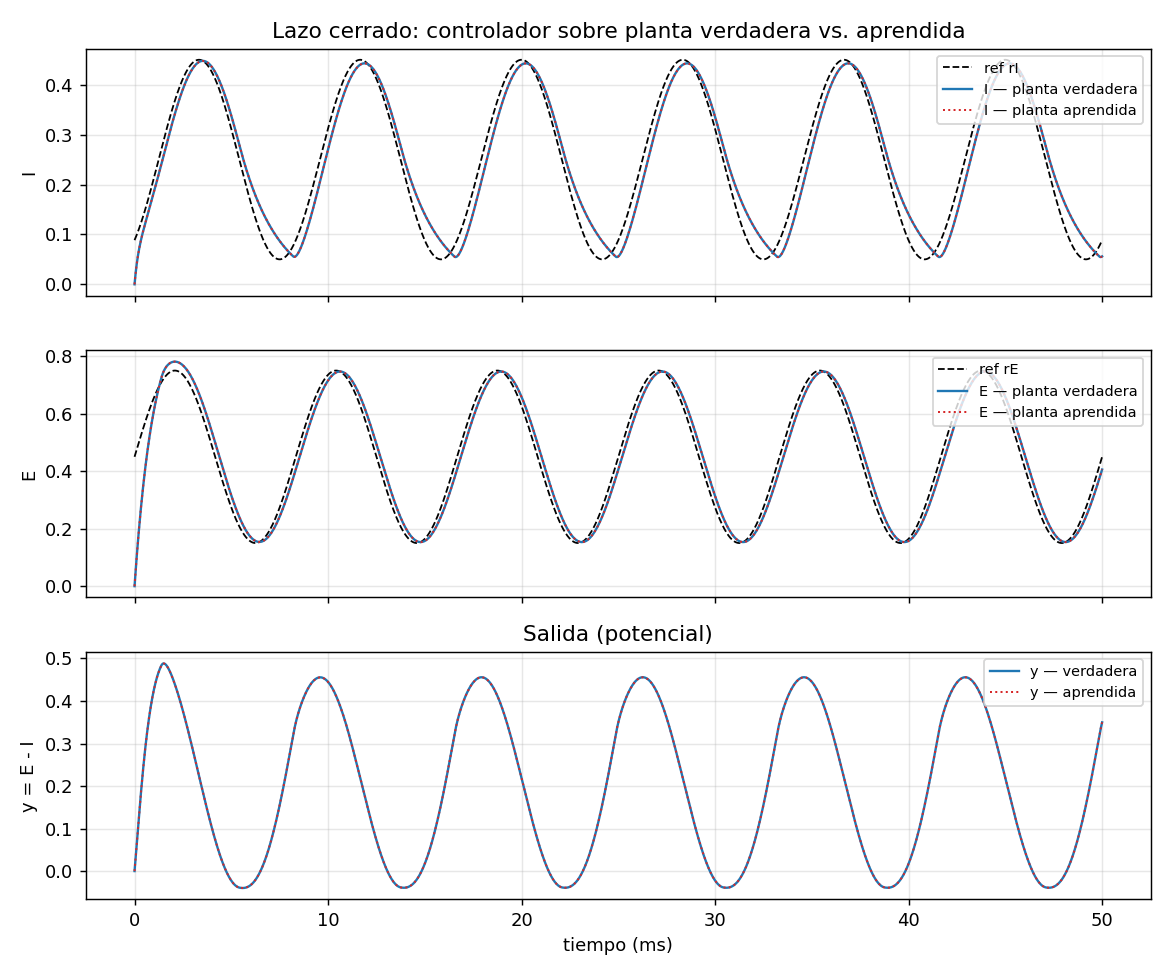
\includegraphics[width=0.8\linewidth]{closed_loop_compare.png}
\caption{Control en lazo cerrado (IMC): seguimiento del ritmo objetivo con parámetros identificados $\hat\theta$ vs.\ parámetros reales. El RMSE es casi idéntico, aun con $\hat\theta$ degradado. \emph{(figura del proyecto)}}
\label{fig:control}
\end{figure}

\paragraph{Por qué importa.} Es el resultado más importante del paquete. Cuantifica \textbf{de punta a punta} que la fragilidad de identificar $w_{II}$ \textbf{no llega al control}, y con eso da vuelta la lectura pesimista del cuello de botella: sí, $w_{II}$ es difícil de identificar, pero para la tarea que nos importa (controlar el ritmo) eso \emph{no es un problema}. La razón estructural \--- la acción integral del IMC \--- está en B5. Este resultado es lo que transforma un estudio de identificabilidad en una historia con moraleja útil: no hay que obsesionarse con recuperar perfectamente cada parámetro si el objetivo aguas abajo tolera el error.

\section{Tabla-resumen}
\label{sec:resumen}

\begin{table}[H]
\centering
\small
\begin{tabular}{@{}p{3.3cm} p{5.5cm} p{5.5cm}@{}}
\toprule
\textbf{Experimento} & \textbf{Resultado clave} & \textbf{Novedad} \\
\midrule
Simulador y datasets (\S\ref{sec:sim}) & Banco de pruebas con \emph{ground truth}; librería de estímulos que cubre el espacio de estados. & Excitación persistente materializada como diseño de datasets para WC. \\[4pt]
Identificación en limpio (\S\ref{sec:limpio}) & 4 pesos casi perfecto ($0.42\%$); los \textbf{10 parámetros} con NODE a \textbf{error máx.\ $1.14\%$}. & Identificar los 10 parámetros de WC con una Neural ODE (no solo los 4 pesos). \\[4pt]
Robustez al ruido + Fisher/SVD (\S\ref{sec:ruido}) & $w_{II}$ el peor: $0.8\%\to41\%$ a $\sigma=0.10$; ranking predicho por la FIM y confirmado. & Bucle \textbf{predecir $\to$ confirmar}: la FIM anticipa $w_{II}$ sin entrenar. \\[4pt]
Remedios guiados por FIM (\S\ref{sec:remedios}) & Fijar/regularizar $w_{II}$: resto de $15.9\%\to9.7\%$; fijar un representante mínimo del acople. & Subset selection + regularización + OED aplicados a WC con receta accionable. \\[4pt]
OED ponderado (\S\ref{sec:oed}) & V-shape, óptimo en $\rho=0.5$: $w_{II}$ a $18.7\%$ vs.\ $\ge93\%$ en los extremos. & OED ponderado al cuello de botella; decorrelación + Q-alta, verificado. \\[4pt]
Familia y límite de $dt$ (\S\ref{sec:familia}) & No concluyente; firme: $dt$ grande solo seguro con estímulos suaves. & Caza del confusor (varianza de optimización, estímulos no comparables). \\[4pt]
Costo computacional (\S\ref{sec:costo}) & WC no rígido ($|\lambda_{\max}|\approx0.70$) $\to$ RK4 $dt$ grande $\sim5\times$ más barato. & La rigidez predice el costo \emph{sin correr nada} (gemelo de la FIM). \\[4pt]
Validación de control (\S\ref{sec:control}) & RMSE casi idéntico con $\hat\theta$ vs.\ reales; fragilidad \textbf{no} se propaga. & Cuantificar end-to-end que la fragilidad de $w_{II}$ no llega al control. \\
\bottomrule
\end{tabular}
\caption{Recorrido experimental: experimento $\to$ resultado clave $\to$ novedad.}
\label{tab:resumen}
\end{table}

\paragraph{Cierre.} El arco es simple de contar: se puede identificar WC casi entero, hay un parámetro rebelde ($w_{II}$) que la teoría predice antes de entrenar, se lo puede mitigar de varias formas, y \--- lo decisivo \--- su fragilidad no daña el control. Dos análisis espectrales (FIM para identificabilidad, rigidez para costo) permiten decidir qué recuperar y cuánto cuesta \emph{antes} de gastar cómputo. Para el detalle teórico ver M6 (identificabilidad, SVD, Fisher, OED), M5 (métodos de identificación con su código) y B5 (controlador IMC y por qué es robusto).

\begin{thebibliography}{9}
\bibitem{wc1972} Wilson, H.R.\ \& Cowan, J.D., ``Excitatory and inhibitory interactions in localized populations of model neurons'', \emph{Biophysical Journal} 12(1):1--24, 1972.
\bibitem{chen} Chen, R.T.Q., Rubanova, Y., Bettencourt, J.\ \& Duvenaud, D., ``Neural Ordinary Differential Equations'', \emph{NeurIPS}, 2018.
\bibitem{raue} Raue, A.\ et al., ``Structural and practical identifiability analysis of partially observed dynamical models by exploiting the profile likelihood'', \emph{Bioinformatics} 25(15):1923--1929, 2009.
\bibitem{chuhahn} Chu, Y.\ \& Hahn, J., ``Parameter set selection for estimation of nonlinear dynamic systems'', \emph{AIChE Journal} 53(11):2858--2870, 2007.
\bibitem{ljung} Ljung, L., \emph{System Identification: Theory for the User}, 2\textsuperscript{a} ed., Prentice Hall, 1999.
\bibitem{plate} Plate, C.\ et al., ``Optimal experimental design for universal differential equations'', 2024.
\end{thebibliography}

\end{document}
